%----------------------------------------------------------------------------------------
%	PACKAGES AND OTHER DOCUMENT CONFIGURATIONS
%----------------------------------------------------------------------------------------

\documentclass{article}

\usepackage{fancyhdr} % Required for custom headers
\usepackage{lastpage} % Required to determine the last page for the footer
\usepackage{extramarks} % Required for headers and footers
\usepackage[usenames,dvipsnames]{color} % Required for custom colors
\usepackage{graphicx} % Required to insert images
\usepackage{listings} % Required for insertion of code
\usepackage{courier} % Required for the courier font
\usepackage{lipsum} % Used for inserting dummy 'Lorem ipsum' text into the template
\usepackage[utf8]{inputenc}
\usepackage[ngerman]{babel}

% Margins
\topmargin=-0.45in
\evensidemargin=0in
\oddsidemargin=0in
\textwidth=6.5in
\textheight=9.0in
\headsep=0.25in

\linespread{1.1} % Line spacing

% Set up the header and footer
\pagestyle{fancy}
%\lhead{\hmwkAuthorName} % Top left header
\chead{\hmwkClass\ : \hmwkTitle} % Top center head
\rhead{\firstxmark} % Top right header
\lfoot{\lastxmark} % Bottom left footer
\cfoot{} % Bottom center footer
\rfoot{Page\ \thepage\ of\ \protect\pageref{LastPage}} % Bottom right footer
\renewcommand\headrulewidth{0.4pt} % Size of the header rule
\renewcommand\footrulewidth{0.4pt} % Size of the footer rule

\setlength\parindent{0pt} % Removes all indentation from paragraphs

%----------------------------------------------------------------------------------------
%	CODE INCLUSION CONFIGURATION
%----------------------------------------------------------------------------------------

\definecolor{MyDarkGreen}{rgb}{0.0,0.4,0.0} % This is the color used for comments
\lstloadlanguages{Perl} % Load Perl syntax for listings, for a list of other languages supported see: ftp://ftp.tex.ac.uk/tex-archive/macros/latex/contrib/listings/listings.pdf
\lstset{language=Perl, % Use Perl in this example
        frame=single, % Single frame around code
        basicstyle=\small\ttfamily, % Use small true type font
        keywordstyle=[1]\color{Blue}\bf, % Perl functions bold and blue
        keywordstyle=[2]\color{Purple}, % Perl function arguments purple
        keywordstyle=[3]\color{Blue}\underbar, % Custom functions underlined and blue
        identifierstyle=, % Nothing special about identifiers                                         
        commentstyle=\usefont{T1}{pcr}{m}{sl}\color{MyDarkGreen}\small, % Comments small dark green courier font
        stringstyle=\color{Purple}, % Strings are purple
        showstringspaces=false, % Don't put marks in string spaces
        tabsize=5, % 5 spaces per tab
        %
        % Put standard Perl functions not included in the default language here
        morekeywords={rand},
        %
        % Put Perl function parameters here
        morekeywords=[2]{on, off, interp},
        %
        % Put user defined functions here
        morekeywords=[3]{test},
       	%
        morecomment=[l][\color{Blue}]{...}, % Line continuation (...) like blue comment
        numbers=left, % Line numbers on left
        firstnumber=1, % Line numbers start with line 1
        numberstyle=\tiny\color{Blue}, % Line numbers are blue and small
        stepnumber=5 % Line numbers go in steps of 5
}

% Creates a new command to include a perl script, the first parameter is the filename of the script (without .pl), the second parameter is the caption
\newcommand{\perlscript}[2]{
\begin{itemize}
\item[]\lstinputlisting[caption=#2,label=#1]{#1.pl}
\end{itemize}
}

%----------------------------------------------------------------------------------------
%	DOCUMENT STRUCTURE COMMANDS
%	Skip this unless you know what you're doing
%----------------------------------------------------------------------------------------

% Header and footer for when a page split occurs within a problem environment
\newcommand{\enterProblemHeader}[1]{
%\nobreak\extramarks{#1}{#1 continued on next page\ldots}\nobreak
%\nobreak\extramarks{#1 (continued)}{#1 continued on next page\ldots}\nobreak
}

% Header and footer for when a page split occurs between problem environments
\newcommand{\exitProblemHeader}[1]{
%\nobreak\extramarks{#1 (continued)}{#1 continued on next page\ldots}\nobreak
%\nobreak\extramarks{#1}{}\nobreak
}

\setcounter{secnumdepth}{0} % Removes default section numbers
\newcounter{homeworkProblemCounter} % Creates a counter to keep track of the number of problems

\newcommand{\homeworkProblemName}{}
\newenvironment{homeworkProblem}[1][Problem \arabic{homeworkProblemCounter}]{ % Makes a new environment called homeworkProblem which takes 1 argument (custom name) but the default is "Problem #"
\stepcounter{homeworkProblemCounter} % Increase counter for number of problems
\renewcommand{\homeworkProblemName}{#1} % Assign \homeworkProblemName the name of the problem
\section{\homeworkProblemName} % Make a section in the document with the custom problem count
%\enterProblemHeader{\homeworkProblemName} % Header and footer within the environment
}{
%\exitProblemHeader{\homeworkProblemName} % Header and footer after the environment
}

\newcommand{\problemAnswer}[1]{ % Defines the problem answer command with the content as the only argument
\noindent\framebox[\columnwidth][c]{\begin{minipage}{0.98\columnwidth}#1\end{minipage}} % Makes the box around the problem answer and puts the content inside
}

\newcommand{\homeworkSectionName}{}
\newenvironment{homeworkSection}[1]{ % New environment for sections within homework problems, takes 1 argument - the name of the section
\renewcommand{\homeworkSectionName}{#1} % Assign \homeworkSectionName to the name of the section from the environment argument
\subsection{\homeworkSectionName} % Make a subsection with the custom name of the subsection
%\enterProblemHeader{\homeworkProblemName\ [\homeworkSectionName]} % Header and footer within the environment
}{
%\enterProblemHeader{\homeworkProblemName} % Header and footer after the environment
}

%----------------------------------------------------------------------------------------
%	NAME AND CLASS SECTION
%----------------------------------------------------------------------------------------

\newcommand{\hmwkTitle}{Übung\ \#6} % Assignment title
\newcommand{\hmwkDueDate}{Donnerstag,\ 11.\ Dezember\ 2014} % Due date
\newcommand{\hmwkClass}{GPU Computing} % Course/class
\newcommand{\hmwkClassTime}{} % Class/lecture time
\newcommand{\hmwkClassInstructor}{} % Teacher/lecturer
\newcommand{\hmwkAuthorName}{Günther Schindler, Alexander Schnapp, Klaus Naumann} % Your name

%----------------------------------------------------------------------------------------
%	TITLE PAGE
%----------------------------------------------------------------------------------------

\title{
\vspace{2in}
\textmd{\textbf{\hmwkClass:\ \hmwkTitle}}\\
\normalsize\vspace{0.1in}\small{Abgabe\ am\ \hmwkDueDate}\\
\vspace{0.1in}\large{\textit{\hmwkClassTime}}
\vspace{3in}
}

\author{\textbf{\hmwkAuthorName}}
\date{} % Insert date here if you want it to appear below your name

%----------------------------------------------------------------------------------------

\begin{document}

\maketitle

%----------------------------------------------------------------------------------------
%	TABLE OF CONTENTS
%----------------------------------------------------------------------------------------

%\setcounter{tocdepth}{1} % Uncomment this line if you don't want subsections listed in the ToC
\newpage
\tableofcontents
\newpage

%----------------------------------------------------------------------------------------
%	Reading
%----------------------------------------------------------------------------------------

\begin{homeworkProblem} [Reading:Roofline - An Insightful
Visual
Performance
Model for
Multicore
Architectures]

In this paper the author introduces a visual computational model for multicore Architecutures called 'roofline' model.
It relates the operational intensity (mean operations per byte
of DRAM traffic) with an upper bound for performance of
a kernel (Attainable GFlops/s). For that 'roofline' is uses the minimum of Peak Floating-Point Performance (constant) and the Peak memory Bandwith multiplied with the operational intensity (line with postiv slope), so wether the problem is compute-bound or memory-bound.

In that way it tells the user what optimizations should he implement and in what order, by pointing out the limiting factor of perfomance.
Using micro benchmarks he is testing 4 different cournels to apply this model.

The Roofline model seams to be a very clear and easy to aply way for characterizing multicore architures for to find a first starting point for optimizations.

\end{homeworkProblem}
\pagebreak

%----------------------------------------------------------------------------------------
%	REDUCTION - CPU
%----------------------------------------------------------------------------------------

\begin{homeworkProblem} [Reduction - CPU]
In diesem Abschnitte sollte eine \textit{global sum reduction} als sequentielle CPU-Version realisiert werden.

\begin{figure}
	\begin{center}
		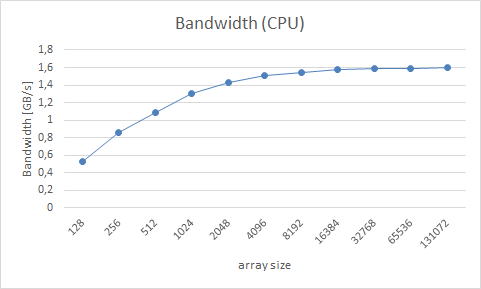
\includegraphics[width=0.8\columnwidth]{cpu.png}
	\end{center}
	\caption{Bandbreite in Abhängigkeit von der Arraygröße für die unoptimierte sequentielle CPU-Version der Global Sum Reduction.}
	\label{fig:abb1} 
\end{figure}

In Abbildung \ref{fig:abb1} sind die Messergebnisse der sequentiellen Implementierung dargestellt. Hier werden alle Elemente des Datentyps \textit{float} eines \textit{arrays} mit Hilfe einer \textit{for-loop} addiert; als Ergebnis erhalten wir die Summe aller Elemente.
\\
\\
Was man in Abbildung \ref{fig:abb1} beobachten kann ist, dass bei einer Größe von 128 Elementen eine Bandbreite von ca. 0,5 \textit{GB/s} gemessen wurde. Mit zunehmender Arraygröße steigt diese bis auf ca. 1,5 \textit{GB/s} an und pendelt sich in diesem Bereich ein. Ab diesem Bereich ist der Cache nicht mehr ausreichend und der Prozess muss auf den Arbeitsspeicher ausweichen, was sich auf die Geschwindigkeit der Berechnung auswirkt.

\end{homeworkProblem}
\pagebreak
%----------------------------------------------------------------------------------------
%	REDUCTION - GPU INITIAL VERSION
%----------------------------------------------------------------------------------------

\begin{homeworkProblem} [Reduction - GPU initial version]
In dieser Aufgabe war das Ziel eine unoptimierte parallele GPU-Version der \textit{global sum reduction} zu implementieren und die Bandbreite in Abhängigkeit der Arraygröße zu messen und diese mit der Bandbreite der CPU-Version zu vergleichen.

\begin{figure}
	\begin{center}
		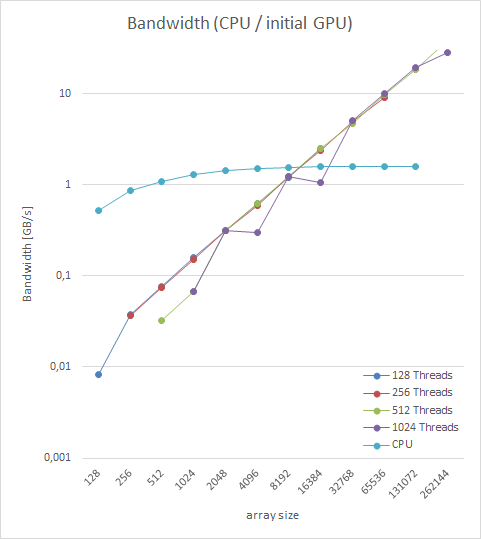
\includegraphics[width=0.8\columnwidth]{cpu_inigpu.png}
	\end{center}
	\caption{Bandbreite in Abhängigkeit von der Arraygröße für die unoptimierte parallele GPU-Version der Global Sum Reduction. Die Messungen wurden mit unterschiedlicher Anzahl von Threads durchgeführt.}
	\label{fig:abb2} 
\end{figure}

Betrachtet man Abbildung \ref{fig:abb2} stellt man fest, dass die sequentielle CPU-Version bis zu einer Arraygröße von knapp über 8192 Elementen eine höhere Bandbreite aufweist, als die unoptimierte parallele GPU-Version. Der Grund hierfür sind der Overhead und die geringe Datenmenge der parallelen Implementierung, welche für kleine Arraygrößen eine negative Auswirkung auf die Bandbreite aufweisen. 
Mit steigenden Problemgrößen steigt auch die Bandbreite der parallelen Implementierung und kann somit zu weitaus schnelleren Ausführungszeiten führen. Dies wirkt sich dementsprechend auch auf den Speed-Up aus.
Aus Gründen der Darstellung wurde hier die Darstellung von Abbildung \ref{fig:abb2} im oberen Bereich begrenzt. Als Peak wurde hier eine Bandbreite von ca. 38 \textit{GB/s} für 262144 Elemente erreicht.  

\end{homeworkProblem}


%----------------------------------------------------------------------------------------
%	REDUCTION - GPU OPTIMIZED VERSION
%----------------------------------------------------------------------------------------

\begin{homeworkProblem} [Reduction - GPU optimized version]
In der letzten Aufgabe dieser Übung sollte eine optimierte parallele GPU-Version der \textit{global sum reduction} implementiert werden und die Bandbreiten aller drei Versionen verglichen werden.

\begin{figure}
	\begin{center}
		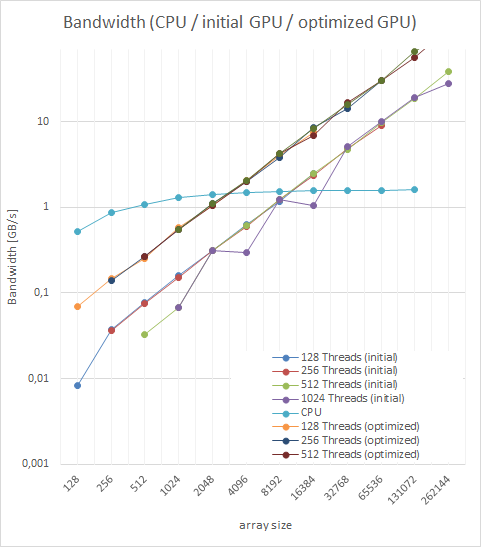
\includegraphics[width=0.8\columnwidth]{cpu_inigpu_optgpu.png}
	\end{center}
	\caption{Bandbreite in Abhängigkeit von der Arraygröße für die unoptimierte als auch die optimierte parallele GPU-Version der Global Sum Reduction. Die Messungen wurden mit unterschiedlicher Anzahl von Threads durchgeführt.}
	\label{fig:abb3} 
\end{figure}

Auf den ersten Blick kann man feststellen, dass die optimierte Version der parallelen Implementierung den \textit{break-even-point} früher - bei einer Arraygröße von ca. 3000 Elementen - erreicht als die unoptimierte Version. Als Maximum konnten wir hier eine Bandbreite von ca. 73 \textit{GB/s} erreichen.

\end{homeworkProblem}
\pagebreak
\end{document}